\subsection{Oberflächenwellen}
% Vrettos2017
% Schmidt2017

\begin{frame}
\frametitle{Video}
\begin{center}

\includegraphics[width=0.2\textwidth]{fig_img/youtube.png}   
\end{center}

\href{https://www.youtube.com/watch?v=6yXgfYHAS7c}{\textsl{Wolfram: Propagation of Seismic Waves: Rayleigh waves}}

\href{https://www.youtube.com/watch?v=t7wJu0Kts7w}{\textsl{Wolfram: Propagation of Seismic Waves: Love waves}}

\end{frame}


\begin{frame}
\frametitle{Rayleigh Wellen}
\begin{figure}
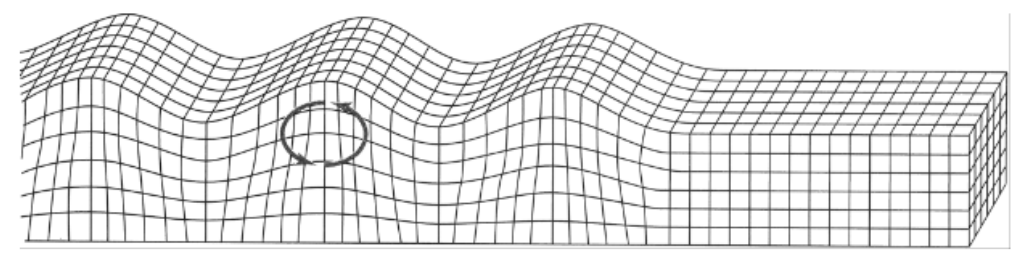
\includegraphics[width=\textwidth]{fig_img/rayleigh_wave} 
\caption*{Kinematik \cite{Vrettos2017}}
\end{figure}

Rayleigh-Wellen sind eine Überlagung von P- und vertikal polarisierter S-Wellen (SV) und werden durch die Halbraumbedingungen ermöglicht.

\end{frame}


\begin{frame}
\frametitle{Rayleigh Wellen}

\begin{figure}
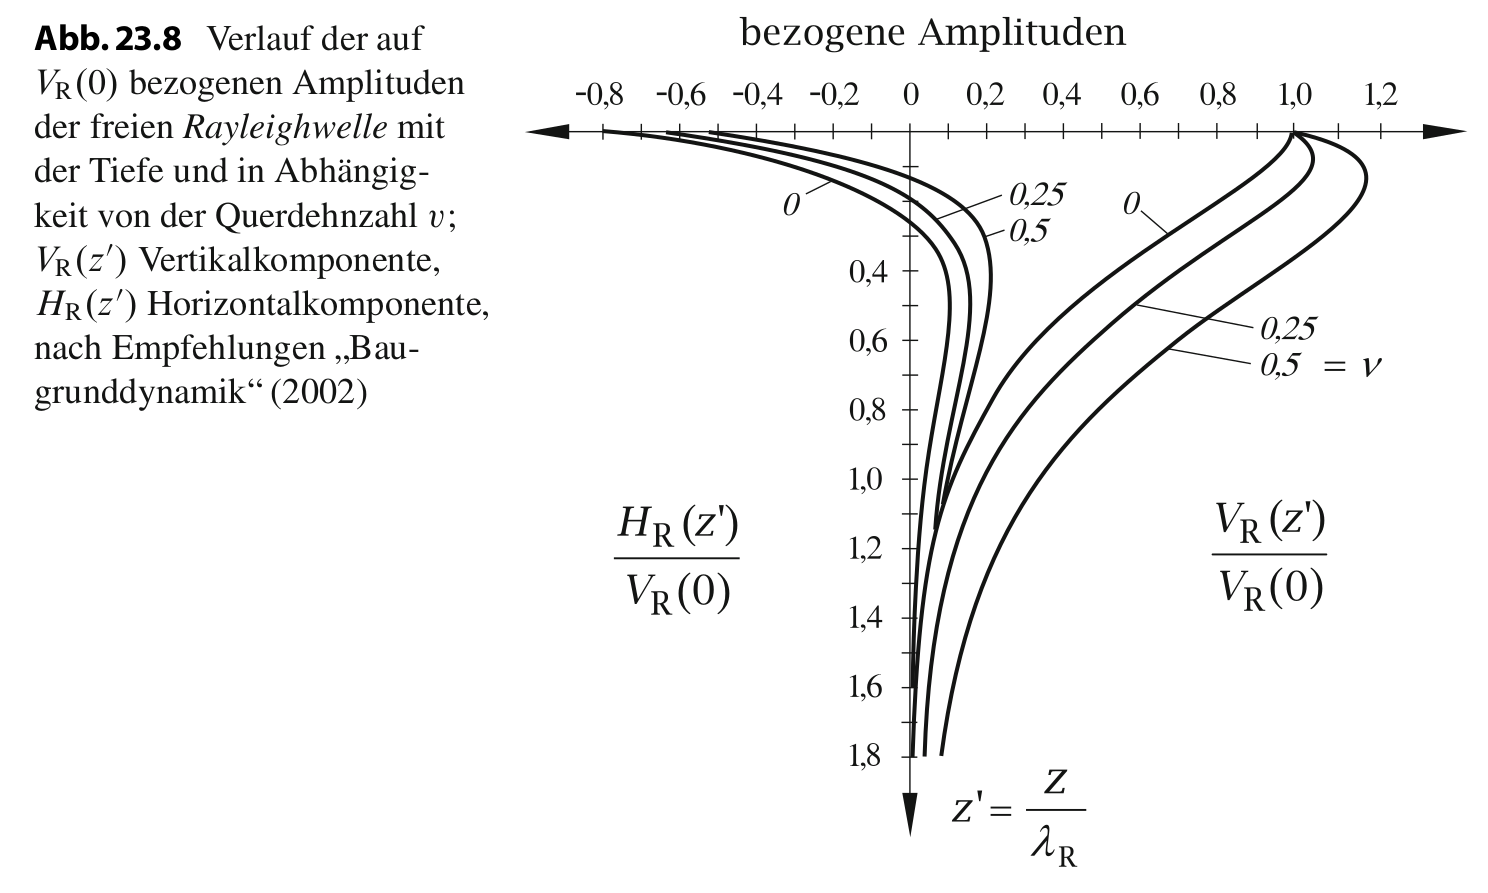
\includegraphics[width=0.8\textwidth]{fig_img/rayleigh_depth} 
\caption*{Exponentielle Abnahme der Amplituden mit der Tiefe \cite{Schmidt2017}}
\end{figure}
\end{frame}


\begin{frame}
\frametitle{Kreisfundament}
\begin{figure}
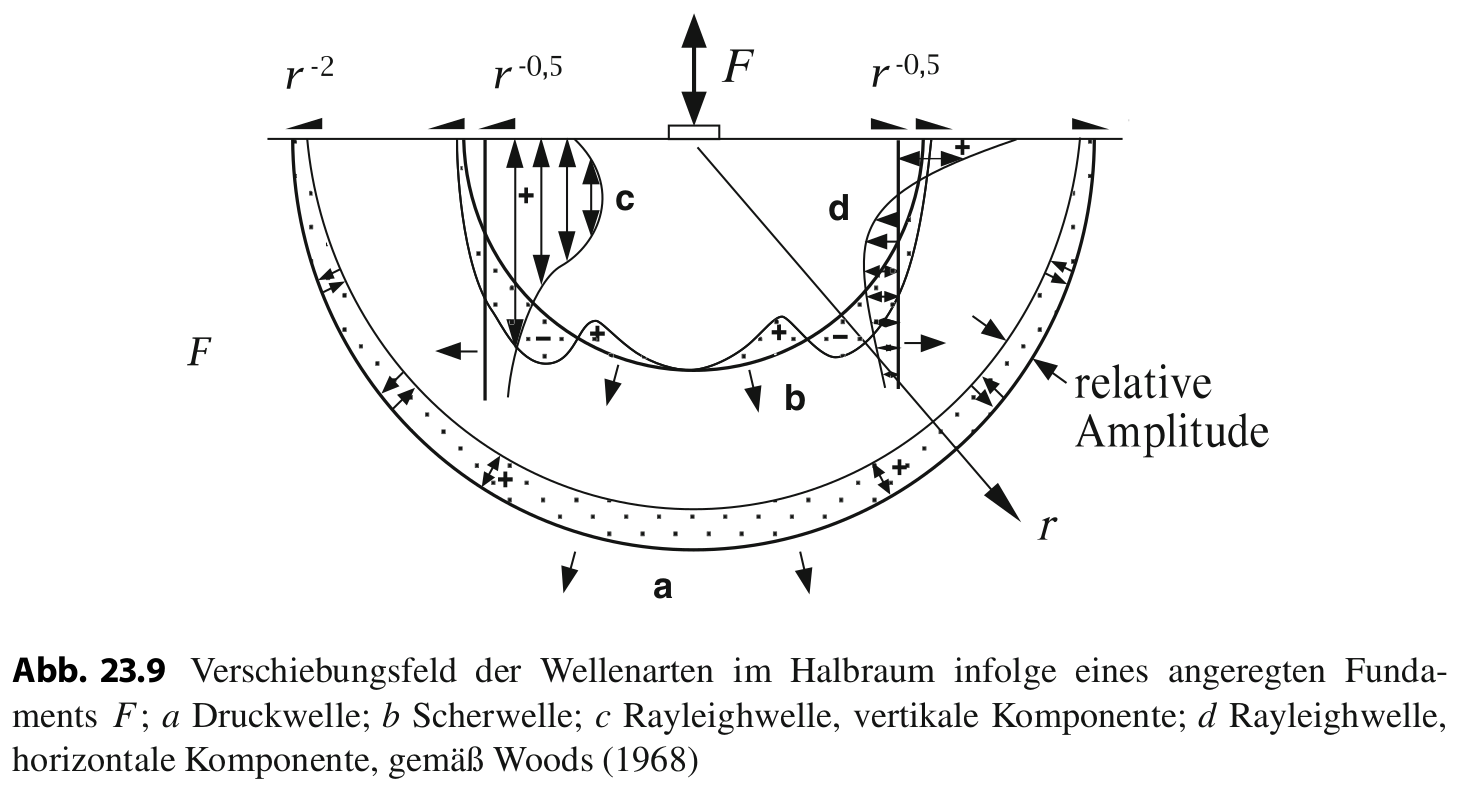
\includegraphics[width=0.9\textwidth]{fig_img/point_load_on_half_space} 
\caption*{Wellenausbreitung unter einem Maschinenfundament \cite{Schmidt2017}}
\end{figure}
\end{frame}


\begin{frame}
\frametitle{Love Wellen}
\only<1>{
\begin{figure}
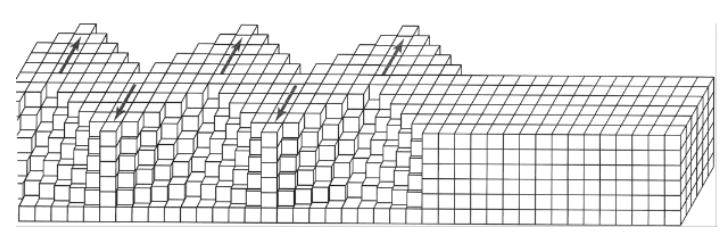
\includegraphics[width=\textwidth]{fig_img/love_wave} 
\caption*{Kinematik \cite{Vrettos2017}}
\end{figure}
Love-Wellen sind eine Überlagung horizontal polarisierter S-Wellen (SH).
}

\only<2>{
\begin{figure}
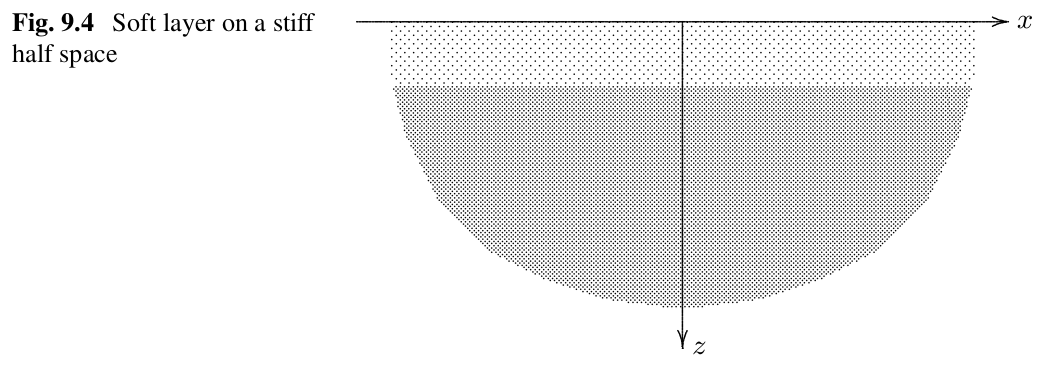
\includegraphics[width=\textwidth]{fig_img/love_wave_configuration} 
\caption*{Love-Wellen sind nur möglich, wenn sich eine weiche Oberflächenschicht auf einem steifen Halbraum befindet \cite{Verruijt2010} und entstehen nur oberhalb eine Grenzfrequenz.}
\end{figure}
Durch Love-Wellen können Erdbeben schwere Zerstörungen anrichten.
}
\end{frame}



